\begin{applicationActivities}

%Short day
\begin{activity}{10}
Consider populations of Green Sunfish (\(G\)) and Bluegills (\(B\)) in the same lake.  They compete for the same food.

\vfill
Which system of ODEs would model this interaction best?
\begin{columns}
\column{0.5\textwidth}
\begin{enumerate}[(A)]
\item 
\begin{alignat*}{2}
\frac{dG}{dt} &= 0.1G-0.002G^2-0.005BG \\
\frac{dB}{dt} &= 0.1B-0.003B^2-0.005BG
\end{alignat*}

\item 
\begin{alignat*}{2}
\frac{dG}{dt} &= 0.1G-0.002G^2-0.005BG \\
\frac{dB}{dt} &= -0.1B-0.003B^2+0.005BG
\end{alignat*}
\end{enumerate}

\column{0.5\textwidth}
\begin{enumerate}
\item[(C)]
\begin{alignat*}{2}
\frac{dG}{dt} &= -0.1G-0.002G^2+0.005BG \\
\frac{dB}{dt} &= 0.1B-0.003B^2-0.005BG
\end{alignat*}

\item[(D)]
\begin{alignat*}{2}
\frac{dG}{dt} &= 0.1G-0.002G^2+0.005BG \\
\frac{dB}{dt} &= 0.1B-0.003B^2+0.005BG
\end{alignat*}
\end{enumerate}
\end{columns}


\end{activity}

\begin{activity}{15}
Consider our Greenfish-Bluegill lake modeled by

\begin{alignat*}{2}
\frac{dG}{dt} &= 0.1G-0.002G^2-0.005BG \\
\frac{dB}{dt} &= 0.1B-0.003B^2-0.005BG
\end{alignat*}

\begin{subactivity}
Plot the isoclines for each species.
\end{subactivity}
\begin{subactivity}
If the lake is stocked with 10 Bluegills and 20 Greenfish, what will happen?
\end{subactivity}
\begin{subactivity}
If the lake is stocked with 25 Bluegills and 5 Greenfish, what will happen?
\end{subactivity}

\end{activity}

\begin{activity}{5}
Plotting the slope field along with the isoclines makes the unstable behavior more clear.
\begin{center}
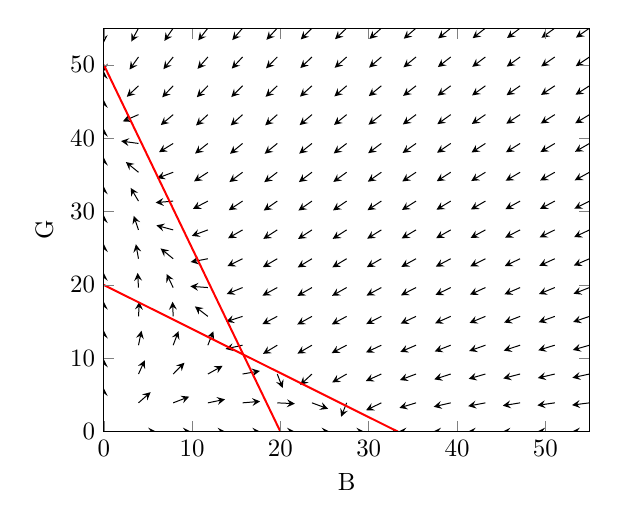
\begin{tikzpicture}[scale=0.9]
    \begin{axis}[
        domain=0:55,
        view={0}{90},
        axis background/.style={fill=white},
		%yticklabels={,,},
		%xticklabels={,,},
		xlabel={B},
		ylabel={G},
		%ticks=none,
    ]
        \addplot3[black,
            quiver={
             u={(0.1*x-0.003*x^2-0.005*x*y)/sqrt(  (0.1*x-0.003*x^2-0.005*x*y)^2+  (0.1*y-0.002*y^2-0.005*x*y)^2)  },
             v={(0.1*y-0.002*y^2-0.005*x*y)/sqrt(  (0.1*x-0.003*x^2-0.005*x*y)^2+  (0.1*y-0.002*y^2-0.005*x*y)^2)},
             scale arrows=2,
            },
            -stealth,samples=15]
                {exp(-x) - 1/2*sin(x) - 1/2*cos(x)};
		\addplot[thick,red] coordinates {(33.3,0) (0,20)};
		\addplot[thick,red] coordinates {(20,0) (0,50)};
    \end{axis}

\end{tikzpicture}
\end{center}

\begin{subactivity}
If the lake is stocked with 20 of each species, what will happen?
\end{subactivity}
\begin{subactivity}
If the lake is stocked with 30 Bluegills and 10 Greenfish, what will happen?
\end{subactivity}
\end{activity}

\end{applicationActivities}
